\documentclass[tikz,border=3pt]{standalone}
\usepackage[T1]{fontenc}
\usepackage{lmodern}
\usetikzlibrary{arrows.meta,calc,positioning,shapes.geometric}

\definecolor{gaNavy}{HTML}{25364B}
\definecolor{gaBlue}{HTML}{0072B2}
\definecolor{gaTeal}{HTML}{009E73}
\definecolor{gaOrange}{HTML}{E69F00}
\definecolor{gaRed}{HTML}{D55E00}
\definecolor{gaGray}{HTML}{6B7280}
\definecolor{gaLight}{HTML}{F4F7F9}

\begin{document}
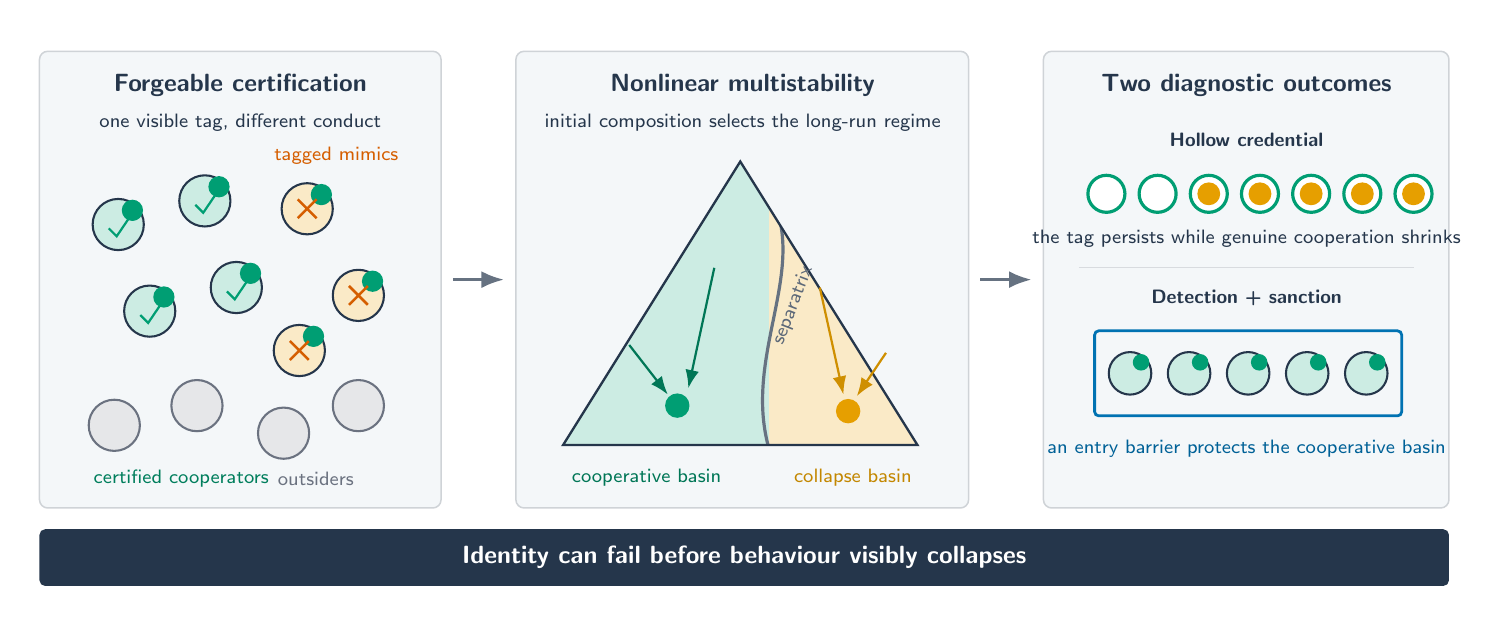
\begin{tikzpicture}[
  x=1cm,y=1cm,
  font=\sffamily,
  >=Latex,
  panel/.style={rounded corners=3pt, draw=gaNavy!22, fill=gaLight,
                line width=.55pt},
  heading/.style={font=\sffamily\bfseries\small, text=gaNavy,
                  align=center},
  smalltext/.style={font=\sffamily\scriptsize, text=gaNavy,
                    align=center},
  agent/.style={circle, minimum size=6.5mm, inner sep=0pt,
                draw=gaNavy, line width=.75pt},
  flow/.style={->, line width=.8pt, draw=gaNavy!70},
]
  \path[use as bounding box] (0,0) rectangle (18.2,7.35);

  % Panel A: a forgeable marker groups cooperators and mimics.
  \draw[panel] (0.15,1.25) rectangle (5.25,7.05);
  \node[heading] at (2.70,6.62) {Forgeable certification};
  \node[smalltext] at (2.70,6.15) {one visible tag, different conduct};

  \foreach \x/\y in {1.15/4.85,2.25/5.15,1.55/3.75,2.65/4.05} {
    \node[agent, fill=gaTeal!20] at (\x,\y) {};
    \draw[fill=gaTeal,draw=none] ($(\x,\y)+(0.18,0.18)$) circle (1.35mm);
    \draw[gaTeal,line width=.8pt] ($(\x,\y)+(-.12,-.05)$) --
      ($(\x,\y)+(-.02,-.15)$) -- ($(\x,\y)+(.17,.13)$);
  }
  \foreach \x/\y in {3.55/5.05,4.20/3.95,3.45/3.25} {
    \node[agent, fill=gaOrange!22] at (\x,\y) {};
    \draw[fill=gaTeal,draw=none] ($(\x,\y)+(0.18,0.18)$) circle (1.35mm);
    \draw[gaRed,line width=.9pt] ($(\x,\y)+(-.12,-.12)$) --
      ($(\x,\y)+(.12,.12)$) ($(\x,\y)+(-.12,.12)$) --
      ($(\x,\y)+(.12,-.12)$);
  }
  \foreach \x/\y in {1.10/2.30,2.15/2.55,3.25/2.20,4.20/2.55} {
    \node[agent, fill=gaGray!17, draw=gaGray] at (\x,\y) {};
  }
  \node[smalltext,text=gaTeal!80!black] at (1.95,1.62) {certified cooperators};
  \node[smalltext,text=gaRed] at (3.92,5.72) {tagged mimics};
  \node[smalltext,text=gaGray] at (3.66,1.62) {outsiders};

  \draw[flow, line width=1.15pt] (5.40,4.15) -- (6.05,4.15);

  % Panel B: nonlinear state space with two basins and a separatrix.
  \draw[panel] (6.20,1.25) rectangle (11.95,7.05);
  \node[heading] at (9.08,6.62) {Nonlinear multistability};
  \node[smalltext] at (9.08,6.15) {initial composition selects the long-run regime};

  \begin{scope}
    \clip (6.80,2.05) -- (9.05,5.65) -- (11.30,2.05) -- cycle;
    \fill[gaTeal!20] (6.60,1.85) rectangle (9.42,5.90);
    \fill[gaOrange!22] (9.42,1.85) rectangle (11.50,5.90);
    \draw[gaNavy!70,line width=1.15pt]
      (9.44,1.92) .. controls (9.05,3.10) and (9.88,4.18) .. (9.48,5.13);
  \end{scope}
  \draw[gaNavy,line width=.85pt] (6.80,2.05) -- (9.05,5.65) --
    (11.30,2.05) -- cycle;
  \node[circle,fill=gaTeal,minimum size=3.1mm,inner sep=0pt] (coop) at (8.25,2.55) {};
  \node[circle,fill=gaOrange,minimum size=3.1mm,inner sep=0pt] (collapse) at (10.42,2.48) {};
  \draw[flow,draw=gaTeal!75!black] (7.64,3.32) -- (8.13,2.69);
  \draw[flow,draw=gaTeal!75!black] (8.72,4.30) -- (8.39,2.77);
  \draw[flow,draw=gaOrange!90!black] (10.06,4.05) -- (10.36,2.69);
  \draw[flow,draw=gaOrange!90!black] (10.90,3.22) -- (10.53,2.67);
  \node[smalltext,text=gaTeal!75!black] at (7.86,1.63) {cooperative basin};
  \node[smalltext,text=gaOrange!85!black] at (10.48,1.63) {collapse basin};
  \node[smalltext,rotate=69,text=gaNavy!75] at (9.72,3.82) {separatrix};

  \draw[flow, line width=1.15pt] (12.10,4.15) -- (12.75,4.15);

  % Panel C: identity deteriorates before aggregate behaviour; enforcement helps.
  \draw[panel] (12.90,1.25) rectangle (18.05,7.05);
  \node[heading] at (15.48,6.62) {Two diagnostic outcomes};

  \node[smalltext,font=\sffamily\bfseries\scriptsize] at (15.48,5.93)
    {Hollow credential};
  \foreach \x in {13.70,14.35,15.00,15.65,16.30,16.95,17.60} {
    \draw[gaTeal,line width=1.15pt,fill=white] (\x,5.24) circle (2.35mm);
  }
  \foreach \x in {15.00,15.65,16.30,16.95,17.60} {
    \fill[gaOrange] (\x,5.24) circle (1.45mm);
  }
  \node[smalltext] at (15.48,4.67)
    {the tag persists while genuine cooperation shrinks};

  \draw[gaNavy!18] (13.35,4.30) -- (17.60,4.30);
  \node[smalltext,font=\sffamily\bfseries\scriptsize] at (15.48,3.92)
    {Detection + sanction};
  \draw[gaBlue,line width=1.0pt,rounded corners=1.5pt]
    (13.55,2.42) rectangle (17.45,3.50);
  \foreach \x in {14.00,14.75,15.50,16.25,17.00} {
    \node[agent,minimum size=5.4mm,fill=gaTeal!20] at (\x,2.96) {};
    \draw[fill=gaTeal,draw=none] ($(\x,2.96)+(0.14,0.14)$) circle (1.05mm);
  }
  \node[smalltext,text=gaBlue!85!black] at (15.48,2.00)
    {an entry barrier protects the cooperative basin};

  \node[rounded corners=2pt,fill=gaNavy,text=white,
        font=\sffamily\bfseries\small,minimum width=17.90cm,
        minimum height=.72cm,align=center] at (9.10,.62)
    {Identity can fail before behaviour visibly collapses};
\end{tikzpicture}
\end{document}
